\section{Methodology Used}
\label{sec:method}

\subsection{Testbed and workloads}
All experiments run in an Ubuntu 24.04 VM (Linux 6.8.0, 4 virtual CPUs (vCPUs), 6\,GiB)
under the macOS Virtualization framework on an Apple M3 Pro. Worker threads
run on CPUs 0--2; the load generator and the trace collector are pinned to
CPU~3. Our benchmark, \texttt{tlbench}, sends requests at random (Poisson)
times from a fixed seed, independent of how fast earlier requests finish
(open loop). Every request has a stable integer id and is served by one of
three worker threads. There are three workloads: \textbf{cpu} (100\,$\mu$s
of fixed computation; the worker is woken through a condition variable);
\textbf{kv}, a small key-value store (8 lookups in a 64\,MiB hash table, a
4\,KiB \texttt{pread} and 20\,$\mu$s of computation, plus a
\texttt{pwrite}+\texttt{fdatasync} every 200 requests); and \textbf{net}
(loopback TCP to epoll-based server threads, 50\,$\mu$s of work, 12
connections). Each runs at three loads (cpu 7/12/17k, kv 30/50/70k, net
10/17/24k requests/s), which keep the workers 17--57\% busy. The generator
spins instead of sleeping: in our pilot runs, a sleeping generator woke up
late and sent requests in bursts, the pitfall Treadmill
describes~\cite{zhang2016treadmill}. Latency is therefore measured from the
moment a request is actually sent until it completes, and the generator's
lateness is logged separately.

\textbf{Noise gate.} In a VM, the host can pause a virtual CPU without the
guest noticing. A small meter, \texttt{hiccup}, spins one thread per vCPU
and records gaps in its own execution. A run starts only when every vCPU
loses less than 5\% of its time (3\% for the first eight runs).

\subsection{Kernel telemetry}
\label{sec:telemetry}
\sys{} attaches tracepoint programs (typed through BTF, the BPF Type Format) to \texttt{sched\_switch},
\texttt{sched\_wakeup[\_new]}, \texttt{sched\_migrate\_task},
\texttt{softirq\_entry/exit} and \texttt{irq\_handler\_entry/exit}. For each
thread of the traced process, a small state machine adds up five kinds of
time: (i)~\emph{preemption wait} ($t_\mathrm{runq}$), from being switched out while still
runnable (the kernel's \texttt{preempt} flag is set or the state is
\texttt{TASK\_RUNNING}) until running again; (ii)~\emph{wakeup delay} ($t_\mathrm{wake}$), from
\texttt{sched\_wakeup} until running; (iii)~\emph{blocked time} ($t_\mathrm{blocked}$), from going
to sleep until the wakeup; (iv)~time on the CPU ($t_\mathrm{oncpu}$); and (v)~hard and soft IRQ
time (interrupt requests, IRQs), charged to the thread that was \emph{interrupted}. It also counts
voluntary and involuntary switches, migrations and interrupts. A wakeup for
a thread that is already running or queued is ignored. The same
programs also update system-wide per-CPU counters (switches, involuntary
switches, wakeups, migrations, interrupts, softirqs per type), which the
collector samples every 5\,ms together with the kernel's pressure-stall
information (PSI). These samples are the \emph{aggregate event-count}
baseline.

\subsection{Matching requests to kernel data}
\label{sec:matching}
Fig.~\ref{fig:arch} shows how the pieces fit together. We compare three ways to find the kernel data that belongs to one request.
\textbf{Uprobe windows} place uprobes on two empty functions,
\texttt{tl\_req\_begin} and \texttt{tl\_req\_end}. The first takes a
snapshot of the thread's counters inside the kernel, and the second sends
one 120-byte record of the differences through a ring buffer. The
application needs no change, but every request costs two traps into the
kernel. \textbf{Per-event streaming} sends every matching scheduler and
interrupt event to user space and joins them afterwards. \textbf{Shared
counters}, the design we propose, keep the per-thread counters in a
\texttt{BPF\_F\_MMAPABLE} array (4096 slots, indexed by thread id mod 4096;
each slot records its owner). The application maps this array into its
memory and copies its own slot with ordinary loads at the start and end of
each request. Because \texttt{bpf\_ktime\_get\_ns} and
\texttt{CLOCK\_MONOTONIC} read the same clock, the application can also add
the part of the current on-CPU stretch that has not been recorded yet. The
kernel does no work per request; it only works when a scheduler or
interrupt event actually touches a traced thread.

\begin{figure}[t]
\centering
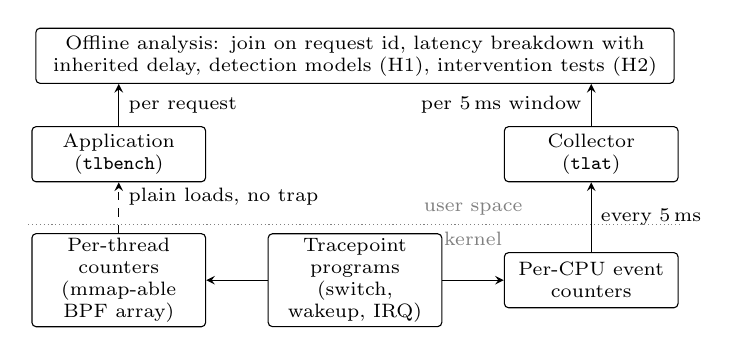
\begin{tikzpicture}[font=\scriptsize, >=stealth,
  box/.style={draw, rounded corners=1.5pt, align=center, inner sep=1.5pt,
              minimum height=0.7cm, text width=2.1cm}]
\node[box] (map)  at (1.2,0)   {Per-thread counters\\(mmap-able BPF array)};
\node[box] (tp)   at (4.2,0)   {Tracepoint programs\\(switch, wakeup, IRQ)};
\node[box] (glob) at (7.2,0)   {Per-CPU event\\counters};
\node[box] (app)  at (1.2,1.6) {Application\\(\texttt{tlbench})};
\node[box] (col)  at (7.2,1.6) {Collector\\(\texttt{tlat})};
\node[box, text width=8.0cm] (ana) at (4.2,2.85)
  {Offline analysis: join on request id, latency breakdown with inherited
   delay, detection models (H1), intervention tests (H2)};
\draw[->] (tp) -- (map);
\draw[->] (tp) -- (glob);
\draw[->, dashed] (map) -- node[pos=0.72, right]{plain loads, no trap} (app);
\draw[->] (glob) -- node[right]{every 5\,ms} (col);
\draw[->] (app) -- node[right]{per request} (app |- ana.south);
\draw[->] (col) -- node[left]{per 5\,ms window} (col |- ana.south);
\draw[gray, densely dotted] (0.05,0.71) -- (8.35,0.71);
\node[gray] at (5.7,0.9) {user space};
\node[gray] at (5.7,0.52) {kernel};
\end{tikzpicture}
\caption{Data path of \sys. Tracepoint programs keep per-thread counters in a
memory-mapped BPF array, which the application reads at request start and
end with no trap; system-wide counters are sampled every 5\,ms as the
aggregate baseline.}
\label{fig:arch}
\end{figure}

\textbf{Validation.} The four time counters come from different
tracepoints, yet for every request they must add up to its service time:
\begin{equation}
t_\mathrm{end}-t_\mathrm{start} = t_\mathrm{oncpu}+t_\mathrm{runq}+t_\mathrm{wake}+t_\mathrm{blocked}.
\label{eq:identity}
\end{equation}

\subsection{Breaking down each request's latency}
A request's latency is split into \emph{sched} (wakeup delay before
service, plus preemption and wakeup waits during service), \emph{irq},
\emph{blocked}, \emph{exec} (on-CPU time minus IRQ time) and \emph{queue}
(time waiting for a free worker). A request can also be late because of an
OS event it never saw: if the request in front of it was preempted, it
waits longer in the queue. We call this \emph{inherited} delay. For request
$i$ and delay type $k \in \{\mathit{sched}, \mathit{irq}, \mathit{blocked}\}$,
\begin{equation}
I_{i,k} = \frac{1}{W} \sum_{j \in C_i} \max\left(0,\; d_{j,k} - 10\,\mu\mathrm{s}\right),
\label{eq:inherited}
\end{equation}
where $C_i$ holds the requests that finished while $i$ waited, $d_{j,k}$ is
their own delay of type $k$, and $W{=}3$ workers; the 10\,$\mu$s floor keeps
many tiny delays from standing in for queue length. The queue time is
then split into inherited sched, irq and blocked parts (capped at the wait)
and a remaining \emph{load} part. A slow request is attributed to the
component that most exceeds the median of the normal requests in the same
run.

\subsection{Detection and attribution analysis}
A request counts as a \emph{tail request} if its latency is above the p99
of separate calibration runs (the median of five runs with seeds
1000--1004, never used for evaluation) for the same workload and load. Each
request has 14 features: 11 counters from its own window and the 3
inherited terms. Times are divided by the tail threshold so that workloads
are comparable, and all features are log-transformed ($\log(1{+}x)$). We
compare a simple rule (total OS delay $>\tau$), logistic regression and a
random forest (150 trees, depth 10), each on three feature sets: the
per-request (\emph{aligned}) features, aggregate counts over 5, 20 or
100\,ms, and a \emph{queue-length control} (the number of requests that
finished during the wait). Models are trained on whole cpu and kv runs
from the main and intervention sets (repetitions 0--2, so stressed runs are
included) and tested on unseen repetitions (3--4) and on the
\textbf{net} workload, which is never used for training or feature design.
Slow requests are rare, so accuracy would be misleading. We report PR-AUC,
the area under the precision--recall curve (a random ranking scores the
fraction of tail requests), with 95\% bootstrap confidence intervals over
runs, plus precision, recall and F1 at the threshold that maximizes F1 on
the training data, and false alarms per minute. To fit in memory we keep
5\% of normal requests and at most 20\,000 tail requests per run, and
weight them back in every metric.

\textbf{Interventions (H2).} At mid load we add one stressor at a time, five
runs each, in random order: a CPU hog on the worker CPUs that runs for 40\%
of every 10\,ms; a softirq flood (UDP over loopback sent from CPU~3, with
Receive Packet Steering (RPS) moving the receive work to CPUs 0--2); an I/O writer (1\,MiB writes
with \texttt{fdatasync}); and an affinity change (a hog on CPU~0 with
workers on CPUs 0--2, compared with workers moved to CPUs 1--2 at 2/3 of
the rate, so that the load per CPU stays the same). Before running them we
wrote down the expected effect of each: hog $\to$ sched, flood $\to$ irq,
I/O $\to$ blocked, moving the workers $\to$ less sched. We then compare the
per-run mean of that delay with the control using a one-sided Mann--Whitney
U test.

\textbf{Reproducibility.} Code, data access and a step-by-step guide with
all tool versions are at
\url{https://github.com/YashvanthSankar/os-course-project};
\texttt{sudo bash scripts/run\_all.sh} reruns all experiments and
regenerates every table and figure.
